%versi 2 (8-10-2016)
\chapter{Landasan Teori}
\label{chap:teori}

\section{Codeigniter}
\label{sec:codeigniter} 
 
\paragraph{} Codeigniter adalah \textit{framework} pengembangan aplikasi untuk \textit{developer} yang membangun situs web menggunakan PHP. Tujuannya adalah untuk memungkinkan Anda mengembangkan proyek lebih cepat, daripada bila \textit{developer} menulis kode dari awal, dengan menyediakan banyak kumpulan \textit{library} untuk tugas-tugas yang sering dibutuhkan dan juga menyediakan tampilan sederhana serta struktur logika untuk mengakses \textit{library-library} tersebut. Codeigniter memungkinkan \textit{developer} untuk fokus secara kretif pada proyek \textit{developer} dengan cara meminimalkan jumlah kode yang dibutuhkan untuk setiap tugas yang diberikan.
\\
\\
Codeigniter dirancang untuk memenuhi kebutuhan :
\begin{itemize}
		\item \textit{Framework} dengan tapak keberadaan yang kecil
		\item performa yang baik
		\item kompabilitas akun \textit{hosting} yang luas yang dapat berjalan di berbagai versi dan konfigurasi PHP
		\item Framework yang hampir tidak membutuhkan konfigurasi
		\item \textit{Framework} yang tidak membutuhkan \textit{command line}
		\item Framework yang tidak mengikuti aturan pengkodean yang ketat
		\item membutuhkan solusi yang sederhana
		\item dokumentasi yang menyeluruh
	\end{itemize}
	
\subsection{Model-View-Controller}
Codeigniter didasari pola pengembangan \textit{Model-View-Controller} atau MVC. MVC memisahkan logika aplikasi dengan tampilannya.
\begin{itemize}
		\item \textbf{\textit{Model}} merepresentasikan struktur data. Pada umumnya kelas-kelas model menampung fungsi-fungsi untuk mengambil, memperbarui atau memasukan data ke dalam basis data.
		\item \textbf{\textit{View}} menampilkan informasi ke pengguna. 
		\item \textbf{\textit{Controller}} berfungsi sebagai perantara antara model dan view.
	\end{itemize}
Codeigniter menerapkan MVC secara longgar karena Model tidak diwajibkan ada. Developer dapat mengembangkan aplikasi dengan hanya menggunakan \textit{View} dan \textit{Controller} saja.

\subsection{Flow Chart Aplikasi}
Gambar dibawah mengilustrasikan aliran data dalam sistem :
\begin{figure} [ht]
	\centering  
	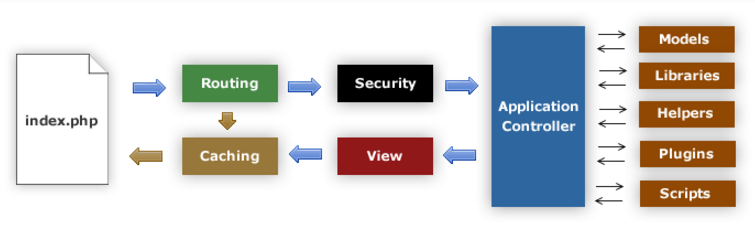
\includegraphics[scale=0.7]{appflowchart.png}  
	\caption[Flow Chart Aplikasi]{Flow Chart Aplikasi} 
	\label{fig:template-jadwal-dosen} 
\end{figure}
\begin{itemize}
		\item index.php berfungsi sebagai controller depan. Menginisialisasi sumber daya yang dibutuhkan untuk menjalankan Codeigniter
		\item Router memeriksa permintaan HTTP untuk menentukan apa yang akan dilakukan pada permintaan tersebut.
		\item Jika ada cache file, maka akan dikirim langsung ke browser. Melewati cara eksekusi sistem yang normal.
		\item Security. Sebelum controller aplikasi dimuat, permintaan HTTP dan data-data pengguna yang telah diserahkan disaring untuk kemanan.
		\item Controller memuat model, pustaka inti (\textit{core libraries}), pembantu dan sumber daya lain yang dibutuhkan untuk memproses permintaan khusus.
		\item Kemudian tampilan akhir dibuat dan dikirim ke web browser untuk dilihat. Jika caching diaktifkan, maka tampilan dimasukan ke dalam cache terlebih dahulu sehingga pada permintaan selanjutnya tampilan tersebut dapat diakses lebih cepat.
	\end{itemize}
	

\section{Zurb Foundation}
\label{zurbfoundation}

\paragraph{}  